\begin{figure}
	\centering
	\pgfplotsset{every axis legend/.append style={
		at={(1.05,0.5)},
		anchor=west}}
	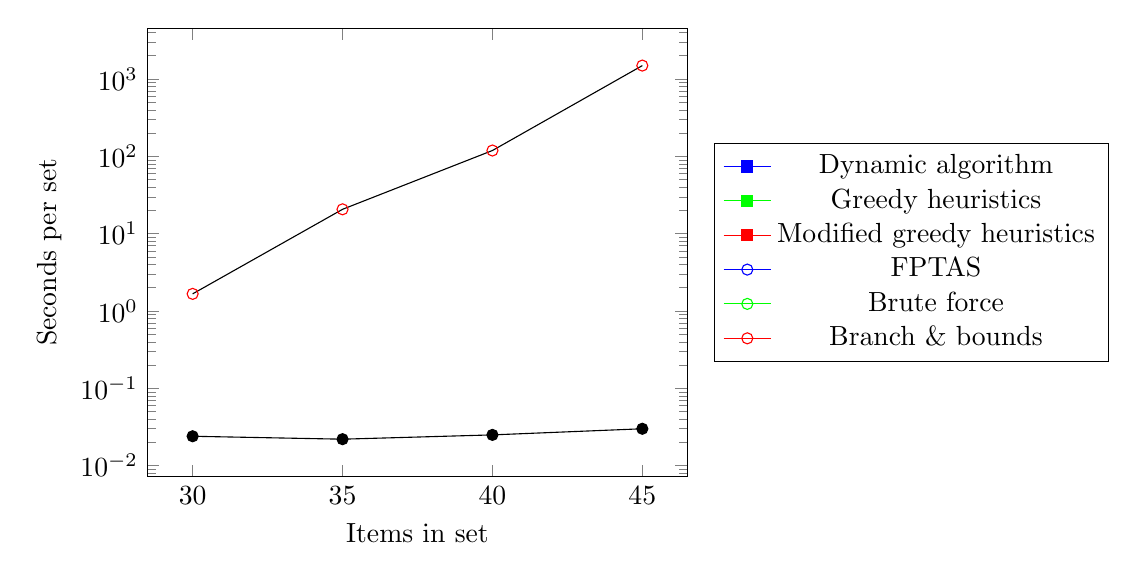
\begin{tikzpicture}
		\begin{semilogyaxis}[
			xlabel=Items in set,
			ylabel=Seconds per set,
			scatter/classes={
				solvePriceDynamic={mark=square*,blue},
				solveHungry={mark=square*,green},
				solveSingle={mark=square*,red},
				fptas={mark=o,blue},
				solveStupid={mark=o,green},
				solveSmart={mark=o,red}
				}
            ]
            
\addplot[scatter,scatter src=explicit symbolic]table[meta=label] {
x y label
30 .024000 genetics
35 .022000 genetics
40 .025000 genetics
45 .030000 genetics
};
\addplot[scatter,scatter src=explicit symbolic]table[meta=label] {
x y label
30 1.666000 solveSmart
35 20.660000 solveSmart
40 118.983000 solveSmart
45 1492.431000 solveSmart
};

			\addlegendentry{Dynamic algorithm}
			\addlegendentry{Greedy heuristics}
			\addlegendentry{Modified greedy heuristics}
			\addlegendentry{FPTAS}
			\addlegendentry{Brute force}
			\addlegendentry{Branch \& bounds}
		\end{semilogyaxis}
	\end{tikzpicture}
\caption{Average time per set with balanced data}
\label{plot:balancedTime}
\end{figure}
